\documentclass{beamer}
\usetheme{Rochester}
\usecolortheme{seagull}
\usepackage{hyperref,verbatim}


\setbeamercovered{transparent}
\setbeamertemplate{navigation symbols}{}
\hypersetup{colorlinks=true,linkcolor=black,urlcolor=blue}


%%%%%%%%%%%%%%%%%%%%%% end of standard headers



\title[]{BCGES short course, session 1, introduction}
\author[]{Vincent Plagnol}
\date{}
\subject{}
\institute{UCL Genetics Institute}


\AtBeginSection[] {
  \begin{frame}
    \frametitle{Outline}
    \tableofcontents[currentsection]
  \end{frame}
}


\begin{document}

\begin{frame}
  \titlepage
\end{frame}


\begin{frame}
  \frametitle{Some technical details about the class}
  \begin{itemize}
  \item Co-taught between myself and Stephane Hue (LSHTM).
  \item My slides and practicals are available on \href{https://github.com/vplagnol/BCGES_short_courses}{Github}.
    \begin{itemize}
    \item This is a collaborative editing side, and I strongly recommend becoming familiar with it.
    \end{itemize}
  \item The practicals all use linux, and some familiarity with the command line will help without being necessary.
    \begin{itemize}
      \item Sections 1-3 of this \href{http://linuxcommand.org/learning_the_shell.php}{manual} should be all you need.
      \item If you struggle with command lines, text editing... spend some extra time this evening to go through this.
    \end{itemize}
  \item Several practicals use the programming language \texttt{R}
    \begin{itemize}
    \item Again, some familiarity would allow you to get more out of the course.
    \end{itemize}
  \end{itemize}
\end{frame}


\begin{frame}
  \frametitle{Key concepts/tools}
  \begin{itemize}
  \item Introduction to vocabulary, concepts
  \item Fastq format
  \item BAM and CRAM format
  \item Using the Galaxy server for basic manipulations
  \end{itemize}
\end{frame}

\begin{frame}
  \frametitle{Outline}
  \tableofcontents
\end{frame}





%%%%%%%%%%%%%%%%%%%%%%%%%%%%%%%%%%%%%%%%%%%%%%%%%%%%%%%%%%%%%%%%%%

\section{Short introduction to sequencing technologies}


\begin{frame}
  \frametitle{The Illumina principle...}
  \begin{center}
    \includegraphics[width=5.5cm]{fig/illumina_workflow.jpg}
  \end{center}
\end{frame}



\begin{frame}
  \frametitle{Illumina paired-end reads}
  \begin{center}
    \includegraphics[width=9cm]{fig/illumina_reads_basic.pdf}
  \end{center}
  \begin{enumerate}
    \item Illumina technology always reads from the 5' end to the 3' end.
    \item If the DNA fragment is shorter than the read length, you get to read the adapter sequence at the end.
    \item If the read length is greater than half the DNA fragment length, fragments overlap in the middle and it is possible to merge into a single synthetic read.
  \end{enumerate}
\end{frame}

\begin{frame}
  \frametitle{Mate-pair is not paired-end}
  \includegraphics[width=10cm]{fig/mate_pair.jpg}
\end{frame}


\begin{frame}
  \frametitle{Read depth}
  \begin{center}
  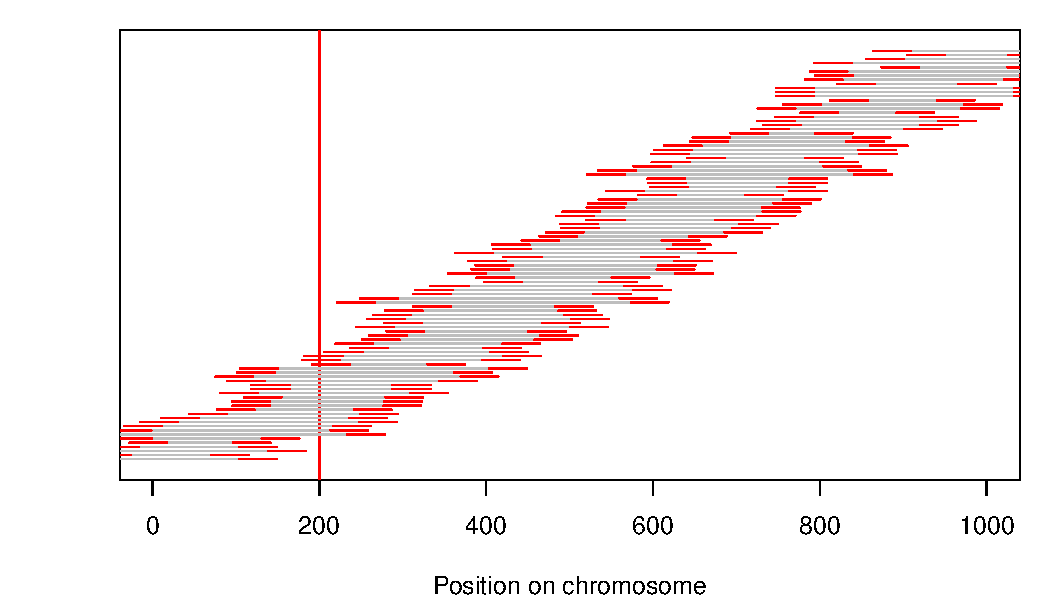
\includegraphics[width=9cm]{fig/entropy_good.pdf}
  \end{center}
\end{frame}


\begin{frame}
  \frametitle{Read depth is a flawed summary of data quality}
  \begin{itemize}
  \item If the depth is uneven, a high mean read depth may not be informative.
  \item Sequence capture technologies introduce a lot of variability in read depth.
  \item So a 30x read depth is to a large extent useful to make sure that a large fraction of the target region (say 90\% of the exome) is covered with at least 10x.
  \item The mean read depth may not need to be as large for a full genome (because of the absence of capture step).
  \end{itemize}
\end{frame}


\begin{frame}
  \frametitle{The read clonality problem}
  \begin{center}
    \only<1>{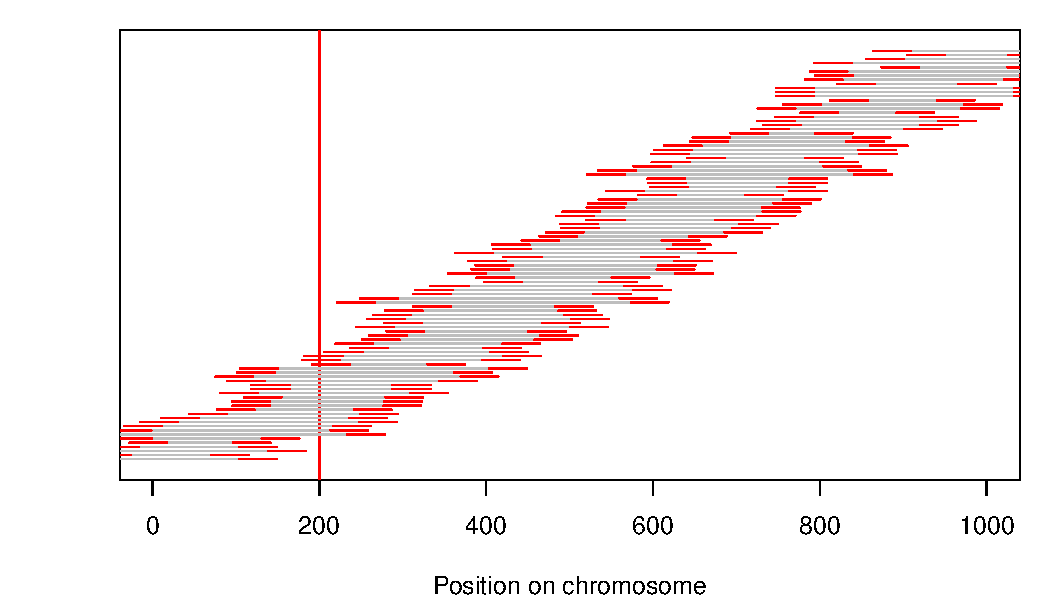
\includegraphics[width=9cm]{fig/entropy_good.pdf}}
    \only<2>{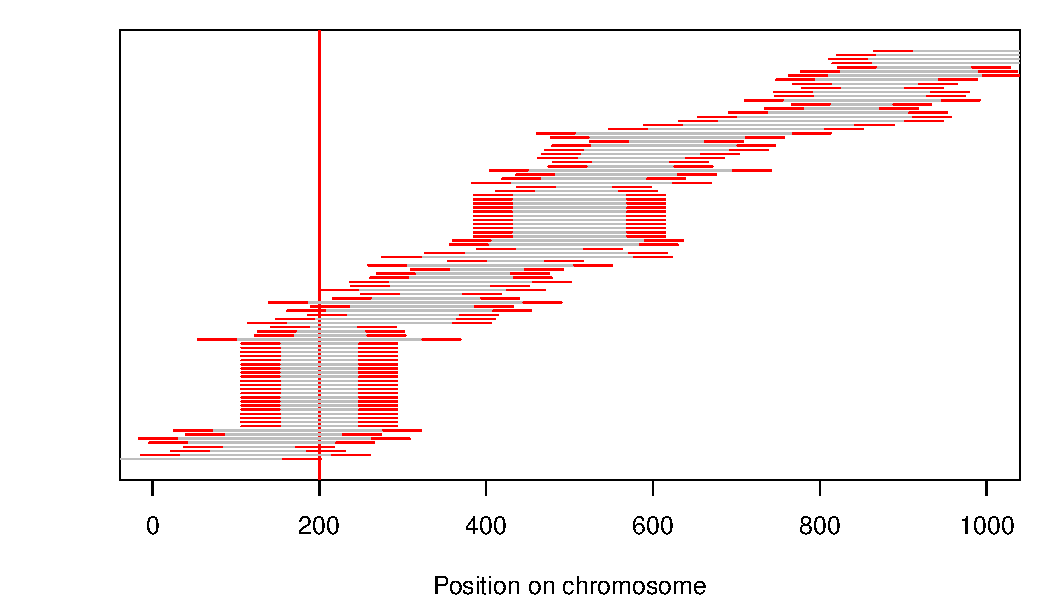
\includegraphics[width=9cm]{fig/entropy_bad.pdf}}
  \end{center}
\end{frame}


\begin{frame}
  \frametitle{Some commonly used vocabulary}
  \begin{itemize}
  \item Index usually referred to a 6-12 bp sequence inserted next to the adapter, which can be used to identify the DNA source (typically the individual being sequenced, but there are more sophisticated things one can do).
  \item Capture refers to the broad range of techniques meant to enrich the DNA for regions of interest (your favorite gene, the exome...).
  \item Hard trimming refers to the cutting of the low(er) quality end of the sequencing read (the 3' end) prior to alignment.
  \item Soft trimming refers to cutting the end(s) of a read at the alignment step, in situations where one does not know what to do with the remaining part.
  \end{itemize}
\end{frame}


\begin{frame}
  \frametitle{Cloud computing}
  \begin{itemize}
  \item There is a lot one can do with Illumina's basespace service.
  \item Remote servers are now available to perform some of these tasks, like the \href{main.g2.bx.psu.edu)}{Galaxy server}
  \item A true solution for cloud computing is the \href{http://aws.amazon.com/ec2}{Amazon server}.
    \begin{itemize}
    \item It takes some expertise but if yuo do not want to set up your own computing environment and want to access an unlimited computing ressource, this is what you want.
    \end{itemize}
  \end{itemize}
\end{frame}


\begin{frame}
  \frametitle{Galaxy servers}
  \begin{itemize}
  \item The main server of Galaxy is located here:  \href{http://main.g2.bx.psu.edu}{http://main.g2.bx.psu.edu}.
  \item But other \href{http://wiki.g2.bx.psu.edu/PublicGalaxyServers?action=show&redirect=Public+Galaxy+Servers}{instances}  exist.
  \item Various Galaxy servers deliver slightly different packages and options.
  \item It is even possible to install your own server if you found it useful.
  \item There are also options for data sharing, and sharing analysis protocols which are really useful.
    \begin{itemize}
    \item The idea is to make the bioinformatic analysis of sequence data more accessible and reproducible.
    \end{itemize}
  \end{itemize}
\end{frame}






%%%%%%%%%%%%%%%%%%%%%%%%%%%%%%
\section{Fastq and BAM format}

\subsection{Fastq format}

\begin{frame}
  \frametitle{Why do we need a fastq format? (1)}
  \begin{itemize}
  \item Best reference:  \href{http://en.wikipedia.org/wiki/FASTQ_format}{Wikipedia page on fastq}.
  \item This is the simplest and most generic flat text format to store sequencing reads of arbitrary size.
    \begin{itemize}
    \item Store the most likely call and a quality associated to it.
    \end{itemize}
  \item A weakness: the second most likely call is not stored.
  \item It is a flat text file so very easy to share across platforms and software.
  \end{itemize}
\end{frame}


\begin{frame}
  \frametitle{Why do we need a fastq format? (2)}
  \begin{itemize}
  \item A typical exome dataset: 43,406,971 reads, each 76bp long.
    \begin{itemize}
    \item That is 3.3 billion bp, hence the size of the human genome,
    \end{itemize}
  \item Each base pair has a quality associated to it, called Phred score.
  \item Storing a number, even an integer is not efficient.
    \begin{itemize}
    \item Typical int format is stored on 32 bits (hence numbers capped by $2^{32}$.
    \item Also we need a text format, more reliable and portable.
    \end{itemize}
  \item The best solution is to store qualities as characters, mapping each ASCII character to its associated number.
  \end{itemize}
\end{frame}


\begin{frame}
  \frametitle{ASCII table}
  \begin{center}
    \includegraphics[width=8cm]{fig/asciifull.jpg}
  \end{center}
\end{frame}



\begin{frame}
  \frametitle{What is a Phred quality meant to be?}
  \begin{itemize}
  \item In an ideal world a quality of $x$ means a probability $10^{- x \slash 10}$ that the call is wrong.
  \item So a completely random call means $75\%$ chances to be wrong.
  \item This more or less matches a minimum score of 2 as $10^{-0.2}$ is equal to 0.63. 
  \item In practice Phred scores are usually poorly calibrated so the interpretation is not straightforward.
    \begin{itemize}
    \item See this \href{http://pathogenomics.bham.ac.uk/blog/2011/07/ion-torrent-316-first-impressions/}{blog post} for example.
    \end{itemize}
  \end{itemize}
\end{frame}

\begin{frame}
  \frametitle{What does the maximum Phred quality mean?}
   \begin{itemize}
   \item Phred scores are typically capped at 40.
   \item It represents a best case scenario of 1/10,000 error rate.
   \item Indeed, of the error was introduced at the PCR stage, the scanner will not capture this information and can give a perfect quality.
   \item As a consequence, the maximum Phred score is a measure of the accuracy of the library preparation, more than the sequencing itself.
   \end{itemize}
\end{frame}


\begin{frame}
  \frametitle{Several flavors of fastq formats}
  \begin{itemize}
  \item The Sanger fastq: qualities = ASCII code - 33
  \item The Illumina fastq: qualities = ASCII code - 64 (mostly historical)
  \item The latest Illumina fastq (CASAVA 1.8): qualities = ASCII code - 33    
    \begin{itemize}
    \item This format adds other technical refinements, including a Y/N flag for each read (Y means failed QC).
    \item Best is to look at some examples and see the differences.
    \end{itemize}
  \end{itemize}
\end{frame}


\begin{frame}
  \frametitle{Splitting the fastq files into smaller chunks}
  \begin{itemize}
   \item Still today, some version of the standard Illumina pipeline splits the fastq into a large number of smaller fastq files.\\
     \includegraphics[width=11cm]{fig/fastq_split.png}
   \item This is apparently useful for the standard CASAVA pipeline that comes with Illumina instruments.
   \end{itemize}
\end{frame}



\begin{frame}
  \frametitle{A useful QC tool for fastq}
  \begin{itemize}
  \item A researcher at the Babraham has put together some tools to check that a fastq file is OK.
  \item See the webpage: \href{http://www.bioinformatics.bbsrc.ac.uk/projects/download.html\#fastqc}{FastQC}
  \item It does some useful checks for base quality, over-representation of k-mers...
  \item It can actually be used within Galaxy, among other things.
  \end{itemize}
\end{frame}

\begin{frame}
  \frametitle{Storage considerations}
  \begin{itemize}
  \item How much a fastq file is of course a function of what is being sequenced.
  \item A standard human exome (38 Mb capture, 30x read depth) will require roughly 8 Gb fastq file.
  \item Compression is key: this storage requirement goes down to 3 Gb after using bzip2 compression.
    \begin{itemize}
    \item Note that bzip2 compression is more effective than gzip.
    \end{itemize}
  \item 1 Tb of data can store roughly 300 human exomes.
  \item Full human sequence is another challenge (easily 200 Gb per sample).
  \end{itemize}
\end{frame}


\begin{frame}
  \frametitle{Illumina internal read QC}
  \begin{itemize}
  \item To remove the least reliable data from the analysis results, often derived from overlapping clusters, raw data is filtered to remove any reads that do not meet the overall quality as measured by the Illumina chastity filter. 
  \item The chastity of a base call is calculated as the ratio of the brightest intensity divided by the sum of the brightest and second brightest intensities.
  \item Clusters pass filter if no more than one base call in the first 25 cycles has a chastity of $>$ 0.6.
  \item Remaining cycles are ignored.
  \item More information on the Illumina support page: \href{http://support.illumina.com/sequencing/sequencing_software/real-time_analysis_rta/questions.ilmn}{Support page}
  \end{itemize}
\end{frame}


%%%%%%%%%%%%%%%%%%%%%%%%%%%%%%%%%
\subsection{BAM, SAM, CRAM}

\begin{frame}
  \frametitle{Outline}
  \tableofcontents[currentsection]
\end{frame}

\begin{frame}
  \frametitle{Why do we need a BAM format?}
  \begin{itemize}
  \item As you will discuss extensively in the rest of this class, we typically want to map the short reads to a known reference genome.
  \item The BAM format is a binary format for storing aligned sequence data
    \begin{itemize}
    \item Which means that it stores the reads plus the alignment position.
    \end{itemize}
  \item BAM is the binary (compressed) version, and an equivalent uncompressed format exists (SAM format).
  \end{itemize}
\end{frame}



\begin{frame}
  \frametitle{The BAM format is sorted and indexed}
  \begin{itemize}
  \item A typical use of a BAM file is to extract information about a specific slice of sequence, not the whole genome or exome.
  \item It is therefore key to be able to access these slices very rapidly, without having to go through the whole file.
  \item To this end, BAM files can be sorted and indexed, which allows constant time access to any fraction of the BAM file.
  \item Best place to learn is the \href{http://samtools.sourceforge.net/SAMv1.pdf}{SAM/BAM reference file}.
  \end{itemize}
\end{frame}


\begin{frame}
  \frametitle{The choice of the reference sequence matters}
  \begin{itemize}
  \item A BAM file is dependent on the sequence it was aligned against.
  \item This information is encoded in the header of the BAM file.
  \item It is useful to get used to reading the headers of BAM files.
    \begin{itemize}
    \item This can be done using \texttt{samtools view -H}.
    \item All the information about what has happened to the BAM file can be found in the headers, as well as the reference genome.
    \end{itemize}
  \end{itemize}
\end{frame}


\begin{frame}
  \frametitle{Basic \texttt{samtools} manipulation}
  \begin{itemize}
  \item It is a good idea to read through the \href{http://samtools.sourceforge.net/samtools.shtml}{samtools} manual.
  \item With the releases of \texttt{samtools} v1.0 and beyond, you should transition toward \href{http://www.htslib.org/}{this location} to update \texttt{samtools}.
  \item Most tools have sophisticated options but \texttt{samtools view} in particular can do useful thing:
    \begin{itemize}
    \item Subset a specific gene/region/chromosome, potentially over the web.
    \item Request specific flags for the reads.
    \end{itemize}
  \end{itemize}
\end{frame}


\begin{frame}
  \frametitle{The flags associated with reads in BAM files}
  \begin{tabular}{lll}
    Flag &       Chr &    Description\\
    \hline
    0x0001   &   p  &     the read is paired in sequencing\\
    0x0002   &   P  &     the read is mapped in a proper pair\\
    0x0004   &   u  &     the query sequence itself is unmapped\\
    0x0008   &   U  &     the mate is unmapped\\
    0x0010   &   r  &     strand of the query (1 for reverse)\\
    0x0020   &   R  &     strand of the mate\\
    0x0040   &   1  &     the read is the first read in a pair\\
    0x0080   &   2  &     the read is the second read in a pair\\
    0x0100   &   s  &     the alignment is not primary\\
    0x0200   &   f  &     the read fails platform/vendor quality checks\\
    0x0400   &   d  &     the read is either a PCR or an optical duplicate
  \end{tabular}
      {\tiny From the \texttt{samtools} manual}
\end{frame}

\begin{frame}
  \frametitle{Even more compression with CRAM}
  \begin{itemize}
  \item CRAM is the next generation version of sequence data storage, meant to optimize storage.
    \begin{itemize}
    \item This is more effective than BAM.
    \item Index is also built-in, which makes sense (who would use a BAM file without its index?)
    \end{itemize}
  \item Here is the \href{http://www.ebi.ac.uk/about/news/service-news/cram-pre-launch}{news release}, with full availability on June 2013.
  \item Recently released version of \texttt{samtools} fully incorporates the BAM format.
  \item More info on CRAM format:
    \begin{itemize}
    \item A scientific \href{http://genome.cshlp.org/content/21/5/734}{paper}.
    \item And a more technical page about the \href{http://www.ebi.ac.uk/ena/about/cram_toolkit}{CRAM} format.
    \end{itemize}
  \end{itemize}
\end{frame}






\end{document}
